%!TEX program = xelatex
\documentclass[color=cyan,mathpazo,titlestyle=hang]{elegantbook}

\author{袁勇}
\email{yongyuanstu@gmail.com}
\zhtitle{基于内容的图像检索}
\zhend{实用手册}
\entitle{Practical Content-based Image Retrieval}
\enend{Handbook}
\version{2.00}
\myquote{一本以实践经验为基础的图像检索指南书}
\logo{logo.pdf}
\cover{cover.pdf}

%green color
   \definecolor{main1}{RGB}{0,120,2}
   \definecolor{seco1}{RGB}{230,90,7}
   \definecolor{thid1}{RGB}{0,160,152}
%cyan color
   \definecolor{main2}{RGB}{0,175,152}
   \definecolor{seco2}{RGB}{239,126,30}
   \definecolor{thid2}{RGB}{120,8,13}
%blue color
   \definecolor{main3}{RGB}{20,50,104}
   \definecolor{seco3}{RGB}{180,50,131}
   \definecolor{thid3}{RGB}{7,127,128}

\usepackage{makecell}
\usepackage{lipsum}
\usepackage{texnames}
\usepackage{url}

%定义python语法高亮%
%开始%
\usepackage{listings}
\usepackage{color}

\definecolor{mygreen}{rgb}{0,0.6,0}
\definecolor{mygray}{rgb}{0.5,0.5,0.5}
\definecolor{mymauve}{rgb}{0.58,0,0.82}

\lstset{ %
  numbers=left,                    %设置显示行号在左边
  frame=topline,                   %让代码周围显示边框
  backgroundcolor=\color{white},   % choose the background color
  basicstyle=\footnotesize,        % size of fonts used for the code
  breaklines=true,                 % automatic line breaking only at whitespace
  captionpos=b,                    % sets the caption-position to bottom
  commentstyle=\color{mygreen},    % comment style
  escapeinside={\%*}{*)},          % if you want to add LaTeX within your code
  keywordstyle=\color{blue},       % keyword style
  stringstyle=\color{mymauve},     % string literal style
}
%结束%


\begin{document}
\maketitle
\tableofcontents
\mainmatter

\chapter{简介}

在Web2.0时代,尤其是随着Flickr、Facebook等社交网站的流行,图像、视频、音频、文本等异构数据每天都在以惊人的速度增长。例如, Facebook注册用户超过10亿,每月上传超过10亿的图片;Flickr图片社交网站2015年用户上传图片数目达7.28亿,平均每天用户上传约200万的图片;中国最大的电子商务系统淘宝网的后端系统上保存着286亿多张图片。针对这些包含丰富视觉信息的海量图片,如何在这些浩瀚的图像库中方便、快速、准确地查询并检索到用户所需的或感兴趣的图像,成为多媒体信息检索领域研究的热点。基于内容的图像检索方法充分发挥了计算机长于处理重复任务的优势,将人们从需要耗费大量人力、物力和财力的人工标注中解放出来。经过十来来的发展,基于内容的图像检索技术已广泛应用于搜索引擎、电子商务、医学、纺织业、皮革业等生活的方方面面。

图像检索按描述图像内容方式的不同可以分为两类,一类是基于文本的图像检索(TBIR, Text Based Image Retrieval),另一类是基于内容的图像检索(CBIR, Content Based Image Retrieval)。

基于文本的图像检索方法始于上世纪70年代,它利用文本标注的方式对图像中的内容进行描述,从而为每幅图像形成描述这幅图像内容的关键词,比如图像中的物体、场景等,这种方式可以是人工标注方式,也可以通过图像识别技术进行半自动标注。在进行检索时,用户可以根据自己的兴趣提供查询关键字,检索系统根据用户提供的查询关键字找出那些标注有该查询关键字对应的图片,最后将查询的结果返回给用户。这种基于文本描述的图像检索方式由于易于实现,且在标注时有人工介入,所以其查准率也相对较高。在今天的一些中小规模图像搜索Web应用上仍有使用,但是这种基于文本描述的方式所带来的缺陷也是非常明显的:首先这种基于文本描述的方式需要人工介入标注过程,使得它只适用于小规模的图像数据,在大规模图像数据上要完成这一过程需要耗费大量的人力与财力,而且随时不断外来的图像在入库时离不开人工的干预;其次,”一图胜千言”,对于需要精确的查询,用户有时很难用简短的关键字来描述出自己真正想要获取的图像;再次,人工标注过程不可避免的会受到标注者的认知水平、言语使用以及主观判断等的影响,因此会造成文字描述图片的差异。

随着图像数据快速增长,针对基于文本的图像检索方法日益凸现的问题,在1992年美国国家科学基金会就图像数据库管理系统新发展方向达成一致共识,即表示索引图像信息的最有效方式应该是基于图像内容自身的。自此,基于内容的图像检索技术便逐步建立起来,并在近十多年里得到了迅速的发展。典型的基于内容的图像检索基本框架如上图1.1所示,它利用计算机对图像进行分析,建立图像特征矢量描述并存入图像特征库,当用户输入一张查询图像时,用相同的特征提取方法提取查询图像的特征得到查询向量,然后在某种相似性度量准则下计算查询向量到特征库中各个特征的相似性大小,最后按相似性大小进行排序并顺序输出对应的图片。基于内容的图像检索技术将图像内容的表达和相似性度量交给计算机进行自动的处理,克服了采用文本进行图像检索所面临的缺陷,并且充分发挥了计算机长于计算的优势,大大提高了检索的效率,从而为海量图像库的检索开启了新的大门。不过,其缺点也是存在的,主要表现为特征描述与高层语义之间存在着难以填补的语义鸿沟,并且这种语义鸿沟是不可消除的。

基于内容的图像检索技术在电子商务、皮革布料、版权保护、医疗诊断、公共安全、街景地图等工业领域具有广阔的应用前景。在电子商务方面,谷歌的Goggles、 阿里巴巴的拍立淘等闪拍购物应用允许用户抓拍上传至服务器端,在服务器端运行图片检索应用从而为用户找到相同或相似的衣服并提供购买店铺的链接;在皮革纺织工业中,皮革布料生产商可以将样板拍成图片,当衣服制造商需要某种纹理的皮革布料时,可以检索库中是否存在相同或相似的皮革布料,使得皮革布料样本的管理更加便捷;在版权保护方面,提供版权保护的服务商可以应用图像检索技术进行商标是否已经注册了的认证管理;在医疗诊断方面,医生通过检索医学影像库找到多个病人的相似部位,从而可以协助医生做病情的诊断……基于内容的图像检索技术已经深入到了许许多多的领域,为人们的生活生产提供了极大的便利。

\section{基于内容的图像检索技术}

\subsection{相同物体图像检索}

相同物体图像检索是指对查询图像中的某一物体,从图像库中找出包含有该物体的图像。这里用户感兴趣的是图像中包含的特定物体或目标,并且检索到的图片应该是包含有该物体的那些图片。如1.3图所示,给定一幅”蒙娜丽莎”的画像,相同物体检索的目标就是要从图像库中检索出那些包含有”蒙娜丽莎”人物的图片,在经过相似性度量排序后这些包含有”蒙娜丽莎”人物的图片尽可能的排在检索结果的前面。相似物体检索在英文文献中一般称为物体检索(Object Retrieval),近似样本搜索或检测(Duplicate Search or Detection)也可以归类于相同物体的检索,并且相同物体检索方法可以直接应用到近似样本搜索或检测上。相同物体检索不论是在研究还是在商业图像搜索产业中都具有重大的价值,比如购物应用中搜索衣服鞋子、人脸检索等。

对于相同物体图像检索,在检索相同的物体或目标时,易受拍摄环境的影响,比如光照变化、尺度变化、视角变化、遮挡以及背景的杂乱等都会对检索结果造成较大的影响,图1.3左图给出了这几种变化的例子,此外,对于非刚性的物体,在进行检索时,物体的形变也会对检索结果造成很大的影响。

由于受环境干扰比较大,因而对于相同物体图像检索,在选取特征的时候,往往会选择那些抗干扰性比较好的不变性局部特征,比如SIFT1、SURF2、ORB3等,并以此为基础通过不同的编码方式构建图像的全局描述,具有代表性的工作有词袋模型4(BoW, Bag of Words)、 局部特征聚合描述符5(VLAD, Vector of Locally Aggregated Descriptors)以及Fisher向量6(FV, Fisher Vector),这一类以类SIFT为基础的图像检索方法,由于结合了类SIFT不变性的特性,并且采用了由局部到全局的特征表达方式,并且在实际应用时在提取SIFT 的时候还可以使用siftGPU加速SIFT提取,因而从整体上来说能够获得比较好的检索效果,但这一类方法通常其特征维度往往是非常高的,如图1.2所示,在牛津建筑物图像数据库上采用词袋模型进行检索,为了获得较高的检索精度,在聚类时聚类数目一般都设置到了几十万,因而其最终表示的特征其维度高达几十万维,因此为它们设计高效的索引方式显得十分必要。

\subsection{相同类别图像检索}

对给定的查询图片,相似图像检索的目标是从图像库中查找出那些与给定查询图像属于同一类别的图像。这里用户感兴趣的是物体、场景的类别,即用户想要获取的是那些具有相同类别属性的物体或场景的图片。为了更好的区分相同物体检索和相同类别检索这两种检索方式区,仍以图1.3左图所举的”蒙娜丽莎”为例,用户如果感兴趣的就是”蒙娜丽莎”这幅画,那么检索系统此时工作的方式应该是以相同物体检索的方式进行检索,但如果用户感兴趣的并不是”蒙娜丽莎”这幅画本身,而是”画像”这一类图片,也就是说,用户所感兴趣的已经是对这幅具体的画进行了类别概念的抽象,那么此时检索系统应该以相同类别检索的方式进行检索。相同类别图像检索目前已广泛应用于图像搜索引擎,医学影像检索等领域。

对于相同类别图像检索,面临的主要问题是属于同一类别的图像类内变化巨大,而不同类的图像类间差异小。如图1.3右图所示,对于”湖泊”这一类图像,属于该类别的图像在表现形式上存在很大的差异,而对于图??????右图下面所示的”dog” 类和”woman”类两张图像,虽然它们属于不同的类,但如果采用低层的特征去描述,比如颜色、纹理以及形状等特征,其类间差异非常小,直接采用这些特征是很难将这两者分开的,因此相同类别图像检索在特征描述上存在着较大的类内变化和较小的类间差异等挑战。近年来,以深度学习(DL, Deep Learning)为主流的自动特征在应用到相同类别图像检索上时,能够极大的提高检索的精度,使得面向相同物体的检索在特征表达方面得到了较好的解决。目前,以卷积神经网络(CNN, Convolutional Neural Network)为主导的特征表达方式也开始在相同物体图像检索上进行展开,并已有了一些相应的工作7,但由于相同物体在构造类样本训练数据时并不像相同类别图像检索那样那么方便,因而相同物体图像检索在CNN模型训练以及抽取自动特征等方面还有待深入。不管是相同物体图像检索还是相同类别图像检索,在使用CNN模型提取自动特征的时候,最终得到的维度一般是4096维的特征,其维度还是比较高的,直接使用PCA等降维的手段,虽然能达到特征维度约减的目的,但在保持必要的检索精度前提下,能够降低的维度还是有限的,因而对于这一类图像检索,同样有必要为它构建够高效合理的快速检索机制,使其适应大规模或海量图像的检索。

\subsection{大规模图像检索特点}

无论是对于相同物体图像检索还是相同类别图像检索,在大规模图像数据集上,它们具有三个典型的主要特征:图像数据量大、特征维度高以及要求相应时间短。下面对这三个主要特征逐一展开说明:

(1) 图像数据量大。得益于多媒体信息捕获、传输、存储的发展以及计算机运算速度的提升,基于内容的图像检索技术经过十几年的发展,其需要适用的图像规模范围也从原来的小型图像库扩大到大规模图像库甚至是海量图像数据集,比如在上世纪九十年代图像检索技术发展的早期阶段,研究者们在验证图像检索算法性能的时候,用得比较多是corel1k,该图像库共1000张图片,与今天同样可以用于图像检索的最流行的图像分类库imageNet数据集相比,其量级已经有了成千上万倍的增长,因而图像检索应满足大数据时代的要求,在大规模图像数据集上应该具备伸缩性。

(2) 特征维度高。图像特征作为直接描述图像视觉内容的基石,其特征表达的好坏直接决定了在检索过程中可能达到的最高检索精度。如果前置特征未表达好,在构建后置检索模型的时候,不但会复杂化模型的构建,增加检索查询的响应时间,而且能够提升的检索精度也是极其有限的。所以在特征提取之初,应该有意识的选取那些比较高层特征。如果将局部特征表达方式也作为”高维”的一种,那么特征的描述能力跟特征的维度高低具有较大的关联,因而在特征描述方面大规模图像检索具有明显的特征维度高的特性,比如词袋模型BoW、VLAD、Fisher向量以及CNN特征。为了对这些高维的特征有一个维度量级的定量认识,本文以词袋模型构建的特征向量为例,在牛津大学建筑物图像数据集上试验了特征维度(在数值上跟聚类单词数目大小相等)对检索精度的影响,从图1.2中可以看到,词袋模型的特征维度是非常高的。因此,面向大规模图像数据集检索的另一个典型特点是图像特征描述向量维度高。

(3) 要求响应速度快。对于用户的查询,图像检索系统应该具备迅速响应用户查询的能力,同时由于大规模图像数据量大、特征维度高,直接采用暴力搜索(Brute Search) 索引策略(也称为线性扫描)难以满足系统实时性的要求,图1.2右图所示的是在牛津大学建筑物图像数据集上平均每次查询所耗费的时间,可以看到在图像数量仅有4063张的牛津大学建筑物图像集,其查询时间在单词数目为100万且重排深度为1000的条件下就需要耗费1 秒左右的时间,并且整个程序还是运行在一台高配的服务器上,因此,大规模图像检索需要解决系统实时响应的问题。

基于哈希的图像检索技术其具体框架如图1.4所示,按步骤可以分为特征提取、哈希编码、汉明距离排序以及重排四个步骤:

(1) 特征提取。对图像数据库中的图像逐一进行特征提取,并将其以图像文件名和图像特征一一对应的方式添加到特征库中;

(2) 哈希编码。哈希编码可以拆分成为两个子阶段,在对特征进行编码之前需要有哈希函数集,而哈希函数集则通过哈希函数学习阶段而得到,因此这两个子阶段分别为哈希函数学习阶段和正式的哈希编码阶段。在哈希函数学习阶段,将特征库划分成训练集和测试集,在训练库上对构造的哈希函数集H(x)=h1(x),h2(x),…,hK(x)H(x)=h1(x),h2(x),…,hK(x) 进行训练学习;正式的哈希编码阶段时,分别将原来的特征xi(i=1,2,…,N)xi(i=1,2,…,N) 代入到学习得到的哈希函数集H(x)H(x) 中,从而得到相应的哈希编码。值得注意的是,如果设计的哈希算法已经经过实验验证有效,那么在实际的应用系统中,在划分数据集的时候,可以将整个图像库既作为训练集也作为图像数据库,从而使得在大规模图像上学到的哈希函数具备较好的适应性;

(3) 汉明距离排序。在汉明距离排序阶段,对于给定的查询图像,逐一计算查询图像对应的哈希编码到其他各个哈希编码之间的汉明距离,然后按从小到大的顺序进行相似性排序,从而得到检索结果;

(4) 重排。针对步骤(3)汉明排序后的结果,可以选择前M(M«N)M(M«N) 个结果或者对汉明距离小于某一设置的汉明距离dcdc 的结果进行重排。一般地,在重排的时候采用欧式距离作为相似性度量得到重排后的结果。因此,从这里可以看到,哈希过程可以看作是筛选候选样本或是粗排序的过程。在采用哈希方法进行大规模图像检索的应用系统中,通常会有重排这一步,但是在设计哈希算法的时候,对性能进行指标评价直接采用的是汉明距离,也就是在评价哈希算法性能的时候,不需要重排这一步。

随着视觉数据的快速增长,面向大规模视觉数据的基于内容的图像检索技术不论是在商业应用还是计算机视觉社区都受到了极大的关注。传统的暴力(brute-force) 搜索方法(又称线性扫描)通过逐个与数据库中的每个点进行相似性计算然后进行排序,这种简单粗暴的方式虽然很容易实现,但是会随着数据库的大小以及特征维度的增加其搜索代价也会逐步的增加,从而使得暴力搜索仅适用于数据量小的小规模图像数据库,在大规模图像库上这种暴力搜索的方式不仅消耗巨大的计算资源,而且单次查询的响应时间会随着数据样本的增加以及特征维度的增加而增加,为了降低搜索的空间的空间复杂度与时间复杂度,在过去的十几年里研究者们找到了一种可供替代的方案— 近似最近邻(ANN, Approximate Nearest Neighbor)搜索方法,并提出了很多高效的检索技术,其中最成功的方法包括基于树结构的图像检索方法、基于哈希的图像检索方法和基于向量量化的图像检索方法。

\chapter{Python及需要的安装包}

要探索计算机视觉世界,首先我们需要安装一些安装包。作为探索计算机视觉之旅的起始,要安装这些安装包特别是OpenCV是非常冗余乏味的,它依赖于你所使用的操作系统。我已经试着将这些安装说明简化成了一份简短的使用指南,不过,正如你所了解的,锁着项目、网站的改变,这些安装说明是会变化的!如果你在安装中遇到了问题,确保查看安装包的网站以获得最新安装说明。

我强力推荐你要么用easy\_install或pip来管理你那些安装包。它会使你的生活变得更简单!

最后,如果你不想自己逐一安装这些安装包的话,我已经预先安装好后所有需要的安装包,并把它们放在一个Ubuntu的虚拟机里。使用该虚拟机可以使你跳过那些繁琐的安装包的安装,直接进入本书的实例中,而不必理会这些安装包的管理、安装说明以及编译错误。

要想获得更多这个预先配置好的虚拟机,可以前往\url{http://www.pyimagesearch.com/practical-python-opencv/}查看详细信息。

现在,让我们来安装这些安装包!

\section{NumPy和SciPy}

NumPy是一个用于Python编程语言的库,它对大型多维数组提供支持。为什么NumPy很重要呢?原因是使用NumPy,我们可以将图像表示为一个多维数组。将图像表示为NumPy数组,不仅易于计算和资源得以有效利用,而且一些其他的图像处理操作和机器学习库也是用NumPy数组来表示的。此外,使用NumPy内置的高水准数学函数,我们能在一幅图像上做快速数值分析。

与NumPy形影不离的是SciPy。SciPy为科学和技术计算提供了更多的支持。

\subsection{Windows}

到目前为止,在你的Windows系统上安装NumPy和SciPy最简单的方式是\url{http://www.scipy.org/install.html}下载并安装二进制分发包。

\subsection{OSX}

如果你运行的是OSX 10.7.0(Lion)或更高版本,NumPy和SciPy已经预先安装好了。

不过,我喜欢安装ScipySuperpack。它包含了最新版的NumPy、SciPy、Matplotlib和其他非常有用的安装包,比如ipython、pandas和scikit-learn。所有的这些安装包是值得安装的,并且如果你在\url{www.PyImageSearch.com}上阅读我的博客,你会发现这些安装包我用得非常的频繁。

\subsection{Linux}

很多Linux发行版,比如Ubuntu,都预先安装有NumPy并且已经是配置好了的。

如果你想要最新版的NumPy和SciPy,你可以从源代码进行编译,不过最简单的方法还是用一个包管理器,比如在Ubuntu上用apt-get。

\section{Matplotlib}

用一句简洁的话概括,matplotlib是一个绘图库。如果你以前用过MATLAB,在matplotlib环境里你很可能会觉得非常的舒适。在分析图像的时候,我们会用到它。不管是画图像直方图还是只是简单地查看图像本身,matplotlib是一个非常有用的工具,你值得将它纳入到你的工具箱中。

\subsection{全平台}

Matplotlib可以在\url{http://matplotlib.org/}上下载。如果你已经安装了ScipySuperpack,那么Matplotlib就已经在你的计算机上安装了。你也可以通过easy\_install或pip来安装它。

此外,在matplotlib官网上还提供了Windows的二进制安装文件。

\section{OpenCV}

如果说NumPy的主要目标是用于有效地表示大型多维数组,那么,OpenCV的主要目标便是实时处理图像。该库从1999年发布以来,已随处可见,直到在2009年发布的第2版中我们才看到了它对NumPy的支持。OpenCV这个库本身是用C/C++写的,但在运行该安装包时它提供了Python的绑定。OpenCV是我手下最喜欢的计算机视觉库,在本书中,我们会经常使用它。

OpenCV的安装是常常会变化的。由于这个库是用C/C++写的,所以在编译的时候需要特别的注意,并要确保预先要安装的东西都已安装。由于OpenCV的最新安装说明是经常会改变的,所以在安装OpenCV时要确保自己去查看OpenCV的网站\url{http://opencv.org/}。

\subsection{Windows和linux}

OpenCV文档提供了在Windows和Linux用二进制版本安装OpenCV非常棒的教程,你可以在这里看到它的安装说明\url{http://docs.opencv.org/doc/tutorials/introduction/table_of_content_introduction/table_of_content_introduction.html#table-of-content-introduction}。

\subsection{OSX}

过去数年,在OSX上安装OpenCV是一件很痛苦的事,幸运的是现在它的安装已变得越来越简单。你需要安装cmake来构建并编译该OpenCV库,你可以从这里下载cmake\href{http://www.cmake.org/cmake/help/install.html}{http://www.cmake.org/cmake/help/install.html}。

安装cmake后,你就可以从SourceForge资源库检查源代码并进行编译。一般情况下,我发觉Guilherme Defreitas关于怎样在OSX上安装OpenCV的说明是非常棒的,并且为OpenCV的学习给出了一个很好的开始。

你可以在这里找到他的说明:\href{http://www.guidefreitas.com/installing-opencv-2-4-2-on-mac-osx-mountain-lionwith-python-support}{http://www.guidefreitas.com/installing-opencv-2-4-2-on-mac-osx-mountain-lionwith-python-support}。

\section{Mahotas}

如OpenCV一样,Mahotas也依赖于NumPy数组。很多在Mahotas中实现的函数都可以在OpenCV中找到,不过在某些情况下,Mahotas接口比OpenCV接口更容易使用,我们将用Mahotas作为OpenCV的补充。

\subsection{全平台}

在不同的平台上安装Mahotas是极其容易的。假设你已经安装了MumPy和SciPy,那么你所有需要做的只是运行pip install mahotas或easy install mahotas。

既然我们已经安装了所有我们需要的安装包,现在就让我们开始探索计算机视觉世界之旅吧!

\subsection{跳过安装}

正如我在前面提到过,安装这些安装包是费时且繁琐的。如果你想跳过上面那些安装过程而直接进入图像处理和计算机视觉世界,我已经打包好了一个预先配置好了的Ubuntu虚拟机,该虚拟机安装好了上面提到的所有安装包。

如果你对该虚拟机感兴趣并且想要下载它的话(它能够节省你很多时间并避免很多麻烦),你可以到这里下载\href{http://www.pyimagesearch.com/practicalpython-opencv/}{http://www.pyimagesearch.com/practicalpython-opencv/}。

\chapter{载入、显示及保存}

这本书的初衷是成为一本实用手册,用于指引怎样用Python和OpenCV来开始计算机视觉编程。本着这样一条信念,那就让我们不要浪费任何时间了。拿起你的键盘开始写些简单的代码,用于从磁盘载入一幅图像,在屏幕上显示它,并将它用不同的格式写入一个文件。在执行该代码的时候,我们的Python脚本应该可以在屏幕上显示我们载入的图像,正如图3.1所示。

首先,我们创建一个名为load\_display\_save.py来包含我们的代码,现在我们可以开始写代码了:

列表 3.1: load\_display\_save.py

\begin{lstlisting}[language=python]
import argparse
import cv2

ap = argparse.ArgumentParser()
ap.add_argument("-i", "--image", required = True,
	help = "Path to the image")
args = vars(ap.parse_args())
\end{lstlisting}

我们要做的第一件事是导入在这个例子中我们需要的包。我们用了argparse来解析我们的命令行参数。然后,导入cv2 - 这里cv2就是我们的OpenCV库,它包含了我们需要的图像处理函数。

\begin{figure}[!hbtp]
\centering  %使图片居中显示
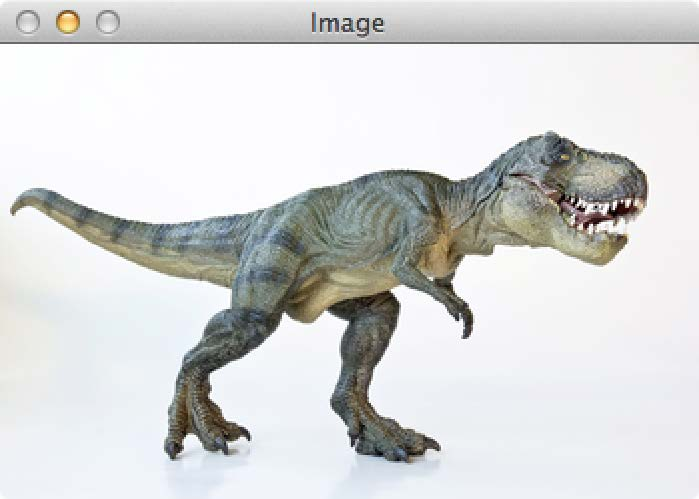
\includegraphics[width=0.8\textwidth]{figure-31.jpg}
\caption{载入并在屏幕上显示一幅霸王龙图像的例子\label{figur:Tyrannosaurus-Rex}}
\end{figure}

上面代码\textbf{第4-7行}用于解析命令行参数。这里我们需要的唯一一个参数是--image:磁盘上图像所在的路径。最后,我们解析这些参数,并在它们保存在一个字典中。

列表 3.2: load\_display\_save.py

\begin{lstlisting}[language=python]
image = cv2.imread(args["image"])
print "width: %d pixels" % (image.shape[1])
print "height: %d pixels" % (image.shape[0])
print "channels: %d" % (image.shape[2])

cv2.imshow("Image", image)
cv2.waitKey(0)
\end{lstlisting}

既然我们有了图像所在的路径,在\textbf{第8行}我们就可以用cv2.imread函数从磁盘载入该图像。cv2.imread函数返回一个NumPy数组,用于表示一幅图像。

\textbf{第9-11行}检查图像的维数。由于图像是用NumPy数组来表示的,我们可以用shape属性来检查该图像的宽、高,以及颜色通道数。

最后,\textbf{第13行}和\textbf{第14行}用于在屏幕上显示实际载入的图像。cv2.imshow的第一个参数是一个字符串,是窗口的“名字”;第二个参数是我们在\textbf{第8行}从磁盘载入的图像。最后调用了cv2.WaitKey函数来暂停运行的脚本,直到我们在键盘上按下一个键。用参数“0”表示按下任意一个键就会释放暂停。

最后,我们将该幅图像以JPG的格式写入文件中:

列表 3.3: load\_display\_save.py

\begin{lstlisting}[language=python]
cv2.imwrite("newimage.jpg", image)
\end{lstlisting}

要运行上面的脚本并显示出图片,我们只需要打开终端窗口,并执行下面的命令:

列表 3.4: load\_display\_save.py

\begin{lstlisting}[language=bash]
$ python load_display_save.py --image ../images/trex.png
\end{lstlisting}

如果不错什么问题的话,你应该可以在你的屏幕上看到\textbf{图3.1}中的霸王龙。要终止脚本的执行的话,只需要在图像窗口上单击,并按下任意键。

检查上面脚本的输出结果,你应该可以看到图片的一些基本信息。你会看到对于那张霸王龙图片,它的宽是350个像素,高是228个像素,以及3个颜色通道(R、G、B三个颜色通道)。用一个NumPy数组表示的话,该数组大小为(350,228,3)。

当我们在写矩阵时,通常我们会将它们写成这种形式:\# 行 $\times$ \#列——但对于NumPy,便不是这样的了。NumPy通常会先给出列数,然后才是行数。这点,你要牢牢记住。

最后,注意文件夹里的内容。你会看到有一个新文件在那儿:newimage.jpg。OpenCV会自动地为我们将PNG格式的图片转换为JPG格式图片!所以在图像格式间进行转换时我们并不需要费什么劲。

下一章,我们将探索怎样在一幅图像上获取像素值并对像素值进行操作。

\chapter{图像基础}

在这一章中,我们将{\color{red}{审查图像的积木}}——像素。我们将详细的讨论什么是像素,以及像素是怎样形成一幅图像的,并且怎么在OpenCV里对这些像素进行操作。

每幅图像由像素集组成。像素是一幅图像的{\color{red}{原材料,积木}}。它是图像的最小单元。

一般情况下,像素通常采用两种方式进行表示:灰度和彩色。在灰度图像中,每一个像素的像素值在0到255之间,“0”代表“黑色”,“1”表示“白色”。

\chapter{特征编码}

局部特征作为一种非常鲁棒性的特征,其与全局特征构成了计算机领域图像内容描述的基础。相比于全局特征,局部特征在刻画图像局部区域的形状、纹理、梯度等方面,往往能够更细的粒度,因而对图像内容的表征也更丰富,但同时也引发了新的问题,即特征处理效率低、存储大等方面的问题。因而需要将局部特征经过某种编码方式,最终表示成一种紧凑的全局特征表示

\section{BoF词袋模型}

基于SIFT局部特征的BOF模型非常适合于做Object retrieval, 下面是自己在oxford building数据库(5063张图片)上进行的一些实验。表格中单词数目为聚类时设定的聚类数目,以及是否采用SIFT或者rootSIFT,rootSIFT怎么计算的可以阅读Object retrieval with large vocabularies and fast spatial matching这篇文章,空间校正即在重排的时候,对错配的SIFT点对进行剔除,剔除的方法可以采用RANSAC或者类RANSAC方法,详细介绍可以阅读SIFT(ASIFT) Matching with RANSAC,检索精度采用平均检索精度(mean Average Precision, mAP),其计算过程可以阅读信息检索评价指标这篇文章。下面需要注意的是查询时间单次查询的结果,并没有进行多次查询进行平均,此外查询时间是查询和计算mAP时间的总和。

\section{VLAD局部聚合向量}

在进行理论分析之前,先来看看VLAD长个什么样子,这里本小子分步展开VLAD是怎么得来的。

提取SIFT特征。对于一个样本数为N的数据库,先对图像库中的所有图像提取SIFT描述子,假设提取到了所有SIFT描述子数目为n,用X来表示的话,X就是一个n*128的矩阵。
聚类生成词汇向量。假设要生成K个单词,对X直接用Kmeans聚成K类,类中心即为单词(也叫码字)。
生成VLAD向量。这一步其实如果对BOW的生成过程清楚的话,这一步理解起来就非常简单了。BoW统计的是描述子落入最近单词里的数目,而VLAD统计的则是这些落入最近单词里与该单词的累积残差。根据Aggregating local image descriptors into compact codes的描述:

BOW做的是描述子的0阶统计分布,而FV则是扩展了的BOW的高阶统计。这里引出来的FV是什么呢?VLAD是FV的特例,这里我们先不关注FV,我们只要借此推得VLAD是BOW的高阶统计就行。

这里我们可以直接调用INRIA开发的Yael工具包,该工具包提供了BoW、VALD以及FV的接口。为了更好的理解VALD编码的过程,可以打开Yael的vlad.c文件,其中有$vlad_compute$方法:

\begin{lstlisting}[language=c++]
void vlad_compute(int k, int d, const float *centroids, 
                  int n, const float *v, float *desc)  
{
  int i,j;
  int *assign = ivec_new (n);
  nn(n, k, d, centroids, v, assign);
  fvec_0 (desc, k * d);
  for (i = 0 ; i < n ; i++) {
    for (j = 0 ; j < d ; j++) 
      desc[assign[i]*d+j] += v[i*d+j] - centroids[assign[i]*d+j];
  }      
  free(assign);
}
\end{lstlisting}

上面清楚的显示了得到的desc(即VLAD特征表示)为距离类中心最近的局部特征的累积和,其中方法nn是做最近邻查找。有了这个接口后,我们要做的就是提取局部特征,比如SIFT,然后使用Yael里提供的KMeans接口做聚类,得到聚类中心,然后调用该函数,即可得到VLAD特征表示。

经过上面三个步骤后,一幅图像可以用一个1(K128)维的向量表示。为了初步验证上面的过程是否正确,来看看上面那篇论文中VLAD的维数是否如这里所理解的是一个1(K128)维的向量,直接看实验表:

\section{Fisher Vector}

\subsection{Fisher核}

在空间$\chi$中,某样本$X$存在$T$个观测变量,记为$X={x_t, t=1 \dots T}$。对应到图像上,样本$X$为图像$I$提取到的$T$个维度为$D$局部特征,比如SIFT。设$\mu_\lambda$为概率密度函数,并且函数包含有$M$个参数,即$\lambda = [\lambda_1, \dots, \lambda_M]$。根据生成式原理,空间样本$\chi$中的元素$X$可以使用该概率密度函数进行建模。在统计学上,分数函数(score funciton)可以由对数似然函数的梯度给出,即:

$$G^X_\lambda = \nabla log \mu_\lambda(X)$$ 

上面对数函数的梯度描述了$M$个参数中,每一个参数$\lambda_i$对该生成式过程的贡献度。

\subsection{Fisher核拓展到图像}

给定图像I,假设从该图像中提取到了$T$个$D$维的局部描述子,比如SIFT,

\begin{lstlisting}[language=c++]
#!/usr/bin/env python
# encoding: utf-8
# Author: yongyuan.name

import os
import multiprocessing
from multiprocessing import Process, freeze_support, Pool


def split_list(alist, wanted_parts=1):
    length = len(alist)
    return [ alist[i*length // wanted_parts: (i+1)*length // wanted_parts]
             for i in range(wanted_parts) ]
             
def cpu_task(img_names, bbin, save_dir):
    for i, line in enumerate(img_names):
        img_path = os.path.join('/home/yuanyong/datasets/oxford', line)
        cmd = bbin + ' ' + img_path + ' ' + save_dir
        os.system(cmd) # returns the exit status
        print "%d(%d), %s" %(i+1, len(img_names), line)

if __name__ == '__main__':

    multiprocessing.freeze_support()
    pool = multiprocessing.Pool()

    parts = 50
    bbin = '/home/yuanyong/cpp/hesaff/hesaff'
    txt_path = '/raid/yuanyong/yael_fv/oxford.txt'
    save_dir = '/raid/yuanyong/yael_fv/oxford_hesaff_sift/'

    with open(txt_path, 'r') as f:
        content = f.readlines()
        content = [x.strip() for x in content]
    blocks = split_list(content, wanted_parts = parts)

    for i in xrange(0, parts):
        pool.apply_async(cpu_task, args=(blocks[i],bbin,save_dir,))
    pool.close()
    pool.join()
\end{lstlisting}

每幅图像由像素集组成。像素是一幅图像的{\color{red}{原材料,积木}}。它是图像的最小单元。

一般情况下,像素通常采用两种方式进行表示:灰度和彩色。在灰度图像中,每一个像素的像素值在0到255之间,“0”代表“黑色”,“1”表示“白色”。

\chapter{ANN搜索}

\section{矩阵相乘}

\section{基于树的方法}

几乎所有的ANN方法都是对全空间的划分,所以基于树的方法也不例外。基于树的方法采用树这种数据结构的方法来表达对全空间的划分,其中又以KD树最为经典。下面左图是KD树对全空间的划分过程,以及用树这种数据结构来表达的一个过程。

对KD树选择从哪一维度进行开始划分的标准,采用的是求每一个维度的方差,然后选择方差最大的那个维度开始划分。这里有一个比较有意思的问题是:为何要选择方差作为维度划分选取的标准?我们都知道,方差的大小可以反映数据的波动性。方差大表示数据波动性越大,选择方差最大的开始划分空间,可以使得所需的划分面数目最小,反映到树数据结构上,可以使得我们构建的KD树的树深度尽可能的小。为了更进一步加深对这一点的认识,可以以一个简单的示例图说明:

假设不以方差最大的x轴为划分面($$x_var = 16.25$$),而是以y轴($$y_var = 0.0$$)轴为划分面,如图中虚线所示,可以看到,该划分使得图中的四个点都落入在同一个子空间中,从而使得该划分成为一个无效的划分,体现在以树结构上,就是多了一层无用的树深度。而以x轴为初始划分则不同(图像实线所示),以x轴为初始划分可以得到数据能够比较均匀的散布在左右两个子空间中,从而使得整体的查找时间能够最短。注意,在实际的kd树划分的时候,并不是图中虚线所示,而是选取中值最近的点。上面示意图构建的具体kd树如下所示:

一般而言,在空间维度比较低的时候,KD树是比较高效的,当空间维度较高时,可以采用下面的哈希方法或者矢量量化方法。

\section{哈希方法}

哈希,顾名思义,就是将连续的实值散列化为0、1的离散值。在散列化的过程中,对散列化函数(也就是哈希函数)有一定的要求。根据学习的策略,可以将哈希方法分为无监督、有监督和半监督三种类型。在评估某种哈希方法用于图像检索的检索精度时,可以使用knn得到的近邻作为ground truth,也可以使用样本自身的类别作为ground truth。所以在实际评估准确度的时候,根据ground truth的定义,这里面是有一点小的trick的。通常对于无监督的哈希图像检索方法,由于我们使用的都是未标记的数据样本,所以我们会很自然的采用knn得到的近邻作为ground truth,但是对于图像检索的这一任务时,在对哈希函数的构造过程中,通常会有“相似的样本经编码后距离尽可能的近,不相似的样本编码后则尽可能的远”这一基本要求,这里讲到的相似,指语义的相似,因而你会发现,编码的基本要求放在无监督哈希方法里,似乎与采用knn得到的近邻作为ground truth的评价方式有些南辕北辙。对无监督哈希方法的ground truth一点小的疑惑在小白菜读书的时候就心存这样的困惑,一直悬而未解。当然,在做无监督的图像哈希方法,采用样本自身的类别作为ground truth是毋庸置疑的。

小白菜读书那会儿,研究了很多的哈希图像检索方法(见hashing-baseline-for-image-retrieval),有时候总会给一些工程实践上的错觉(在今天看来是这样的),即新论文里的方法远远碾压经典的方法,那是不是在实际中这些方法就很work很好使。实践的经历告诉小白菜,还是经典的东西更靠谱,不是因为新的方法不好,而是新的事物需要经过时间的沉淀与优化。

所以,这里不会对近两年的哈希方法做铺陈,而是聊一聊工程中在要使用到哈希方法的场景下一般都会选用的局部敏感哈希(Local Sensitive Hashing, LSH)。

\section{矢量量化方法}

矢量量化方法,即vector quantization,其具体定义为:将一个向量空间中的点用其中的一个有限子集来进行编码的过程。在矢量量化编码中,关键是码本的建立和码字搜索算法。比如常见的聚类算法,就是一种矢量量化方法。而在ANN近似最近邻搜索中,向量量化方法又以乘积量化(PQ, Product Quantization)最为典型。在之前的博文基于内容的图像检索技术的最后,对PQ乘积量化的方法做过简单的概要。在这一小节里,小白菜结合自己阅读的论文和代码对PQ乘积量化、倒排乘积量化(IVFPQ)做一种更加直观的解释。

\subsection{PQ乘积量化}

PQ乘积量化的核心思想还是聚类,或者说具体应用到ANN近似最近邻搜索上,K-Means是PQ乘积量化子空间数目为1的特例。PQ乘积量化生成码本和量化的过程可以用如下图示来说明:

在训练阶段,针对N个训练样本,假设样本维度为128维,我们将其切分为4个子空间,则每一个子空间的维度为32维,然后我们在每一个子空间中,对子向量采用K-Means对其进行聚类(图中示意聚成256类),这样每一个子空间都能得到一个码本。这样训练样本的每个子段,都可以用子空间的聚类中心来近似,对应的编码即为类中心的ID。如图所示,通过这样一种编码方式,训练样本仅使用的很短的一个编码得以表示,从而达到量化的目的。对于待编码的样本,将它进行相同的切分,然后在各个子空间里逐一找到距离它们最近的类中心,然后用类中心的id来表示它们,即完成了待编码样本的编码。

正如前面所说的,在矢量量化编码中,关键是码本的建立和码字的搜索算法,在上面,我们得到了建立的码本以及量化编码的方式。剩下的重点就是查询样本与dataset中的样本距离如何计算的问题了。

在查询阶段,PQ同样在计算查询样本与dataset中各个样本的距离,只不过这种距离的计算转化为间接近似的方法而获得。PQ乘积量化方法在计算距离的时候,有两种距离计算方式,一种是对称距离,另外一种是非对称距离。非对称距离的损失小(也就是更接近真实距离),实际中也经常采用这种距离计算方式。下面过程示意的是查询样本来到时,以非对称距离的方式(红框标识出来的部分)计算到dataset样本间的计算示意:


具体地,查询向量来到时,按训练样本生成码本的过程,将其同样分成相同的子段,然后在每个子空间中,计算子段到该子空间中所有聚类中心得距离,如图中所示,可以得到4*256个距离,这里为便于后面的理解说明,小白菜就把这些算好的距离称作距离池。在计算库中某个样本到查询向量的距离时,比如编码为(124, 56, 132, 222)这个样本到查询向量的距离时,我们分别到距离池中取各个子段对应的距离即可,比如编码为124这个子段,在第1个算出的256个距离里面把编号为124的那个距离取出来就可,所有子段对应的距离取出来后,将这些子段的距离求和相加,即得到该样本到查询样本间的非对称距离。所有距离算好后,排序后即得到我们最终想要的结果。

从上面这个过程可以很清楚地看出PQ乘积量化能够加速索引的原理:即将全样本的距离计算,转化为到子空间类中心的距离计算。比如上面所举的例子,原本brute-force search的方式计算距离的次数随样本数目N成线性增长,但是经过PQ编码后,对于耗时的距离计算,只要计算4*256次,几乎可以忽略此时间的消耗。另外,从上图也可以看出,对特征进行编码后,可以用一个相对比较短的编码来表示样本,自然对于内存的消耗要大大小于brute-force search的方式。

在某些特殊的场合,我们总是希望获得精确的距离,而不是近似的距离,并且我们总是喜欢获取向量间的余弦相似度(余弦相似度距离范围在[-1,1]之间,便于设置固定的阈值),针对这种场景,可以针对PQ乘积量化得到的前top@K做一个brute-force search的排序。

\subsection{倒排乘积量化}

倒排PQ乘积量化(IVFPQ)是PQ乘积量化的更进一步加速版。其加速的本质逃不开小白菜在最前面强调的是加速原理:brute-force搜索的方式是在全空间进行搜索,为了加快查找的速度,几乎所有的ANN方法都是通过对全空间分割,将其分割成很多小的子空间,在搜索的时候,通过某种方式,快速锁定在某一(几)子空间,然后在该(几个)子空间里做遍历。在上一小节可以看出,PQ乘积量化计算距离的时候,距离虽然已经预先算好了,但是对于每个样本到查询样本的距离,还是得老老实实挨个去求和相加计算距离。但是,实际上我们感兴趣的是那些跟查询样本相近的样本(小白菜称这样的区域为感兴趣区域),也就是说老老实实挨个相加其实做了很多的无用功,如果能够通过某种手段快速将全局遍历锁定为感兴趣区域,则可以舍去不必要的全局计算以及排序。倒排PQ乘积量化的”倒排“,正是这样一种思想的体现,在具体实施手段上,采用的是通过聚类的方式实现感兴趣区域的快速定位,在倒排PQ乘积量化中,聚类可以说应用得淋漓尽致。

倒排PQ乘积量化整个过程如下图所示:

在PQ乘积量化之前,增加了一个粗量化过程。具体地,先对N个训练样本采用K-Means进行聚类,这里聚类的数目一般设置得不应过大,一般设置为1024差不多,这种可以以比较快的速度完成聚类过程。得到了聚类中心后,针对每一个样本$x_i$,找到其距离最近的类中心$c_i$后,两者相减得到样本$x_i$的残差向量($x_i-c_i$),后面剩下的过程,就是针对($x_i-c_i$)的PQ乘积量化过程,此过程不再赘述。

在查询的时候,通过相同的粗量化,可以快速定位到查询向量属于哪个$c_i$(即在哪一个感兴趣区域),然后在该感兴趣区域按上面所述的PQ乘积量化距离计算方式计算距离。

\section{拓展查询}

拓展查询(QE, Query Expansion): 指对返回的前top@K个结果,包括查询样本本身,对它们的特征求和取平均,再做一次查询,此过程称为拓展查询。

从上面的定义可以看出,拓展查询属于重排的一种方式。通过Query Expansion,以达到提高检索召回率的目的。前面的博文RANSAC算法做直线拟合曾介绍过RANSAC的基本思想,放在词袋模型里(相应博文见图像检索:BoW图像检索原理与实战),我们可以使用RANSAC方法或Weak Geometry Consistency方法做几何校正,进行重排以提高检索的精度。在这篇博文中,小白菜暂时抛开其他的重排方法,重点分析Query Expansion对图像检索精度的提升。

根据小白菜读图像检索论文获得的对Query Expansion的感知,做完Query Expansion能够获得百分之几的精度提升。为了证实Query Expansion对检索精度的改善,在过去一段时间里,小白菜在Oxford Building数据库上对其做了验证。下面是小白菜对Query Expansion的实验整理和总结。

\bibliographystyle{ieeetr}
\bibliography{reference}
\addcontentsline{toc}{chapter}{参考文献}

\end{document}
